\documentclass{article}
\usepackage[utf8]{inputenc}
\usepackage{fancyhdr}
\usepackage{enumitem}
\usepackage{amsmath}
\usepackage[hidelinks]{hyperref}
\usepackage{url}

\usepackage[]{graphicx}
\usepackage{caption}
\usepackage{subcaption}

\usepackage[section]{placeins}

\usepackage{geometry}
\geometry{margin=0.9in}

\usepackage[bottom]{footmisc}

\usepackage{xcolor}
\usepackage{listings}

\renewcommand\UrlFont{\color{blue}\rmfamily}

\begin{document}

\title{\vspace{-1.5cm}Documentation of New Reference Simulations}

\author{
  Mitchell Burdorf\footnote{\href{mailto:mitchell_burdorf@brown.edu}{mitchell\_burdorf@brown.edu}}
  \and
  Jonathan Pober\footnote{\href{mailto:jonathan_pober@brown.edu}{jonathan\_pober@brown.edu}}
}

\maketitle

%%%%%%%%%%%%%%%%%%%%%%%%%%%%%%%%%%%%%%%%%%%%%%%%%%%%%%%%%%%%%%%%%
%%                            ABSTRACT                         %%
%%%%%%%%%%%%%%%%%%%%%%%%%%%%%%%%%%%%%%%%%%%%%%%%%%%%%%%%%%%%%%%%%
\vspace{-0.8cm}
\begin{abstract}
This memo documents the new first-generation reference simulations. A discussion of each reference simulation is given to provide intuition for simulation output and impetus. Relevant analysis is provided as necessary.
\end{abstract}

\section*{Interferometry Simulation and Axes of Testing}

An antenna array takes data over a range of frequencies, times, and baselines. For each unique time, frequency, and baseline we have a measurement known as a visibility. As the number of baselines scales as the number of antennas squared, the size of simulation output scales rather rapidly as $O(\text{antennas}^2 * \text{times} * \text{frequencies})$. For a simulator, we additionally have to keep track of our model of the sky and our beam model.

We require that pyuvsim is accurate and consistent for a range of inputs along these 5 axes: baseline, frequency, time, source, beam. We do so with the parameters in Table \ref{tab:my_label}. Some of the simulation parameters exist to test a specific interface -- 1.6\_HEALPix -- special location -- 1.8\_lunar -- or simulation capability -- 1.7\_Multi\_Beam and 1.5\_UVBeam. The beam testing occurs across all reference simulations.

\begin{table}[h!]
\setlength\belowcaptionskip{-20pt}
    \centering
    \begin{tabular}{|c|c|c|c|c|c|c}\hline
    Simulation Name & Baseline Layout & Frequencies & Times & Sources & Beam Type\\\hline
    1.1\_Baseline Number & MWA Phase I & 1 & 1 & RASG & Short Dipole\\
    1.2\_Time Axis & Baseline\_Lite\_4x & 1 & 3600 & 2 & Uniform\\
    1.3\_Frequency Axis & Baseline Lite & 10000 & 1 & R & Gaussian\\
    1.4\_Source Axis & 5\_km\_Triangle & 1 & 1 & GLEAM & Airy\\
    1.5\_UVBeam & MWA Phase I & 2 & 2 &  R & MWA UVBeam\\
    1.6\_HEALPix & Baseline Lite & 1 & 1 & GSM 128 & Airy\\
    1.7\_Multi\_Beam & Baseline Lite & 100 & 100 & R & All 4 Analytic\\
    1.8\_Lunar & MWA Phase I & 1 & 1 & MOON & Uniform\\
    \hline\end{tabular}
    \caption{Table of new reference simulation configurations. A number is simply the number of points, and other descriptions are as follows: MWA Phase I is a relatively complex antenna layout also known as 128T with 128 antennas, and Baseline Lite and Baseline Lite 4x are simple layouts with only 4 antennas --- see Figure \ref{fig:arrays}. Short Dipole, Uniform, Airy, and Gaussian beams are analytic beams, and MWA UVBeam is a non-analytic beam created from an electromagnetic simulation of the MWA beam. "RASG", "R", and "MOON" are text catalogs of point sources that spell out those letters on the sky --- see Figure \ref{fig:arrays}. "GLEAM" is a large skymodel of the south sky, and "GSM 128" is a HEALPix map with nside 128 created with pygdsm and healpy.}
    \label{tab:my_label}
\end{table}


%%%%%%%%%%%%%%%%%%%%%%%%%%%%%%%%%%%%%%%%%%%%%%%%%%%%%%%%%%%%%%%%%
%%                        Section 1                            %%
%%%%%%%%%%%%%%%%%%%%%%%%%%%%%%%%%%%%%%%%%%%%%%%%%%%%%%%%%%%%%%%%%

\section*{New Reference Simulations}

We briefly introduce each new simulation and provide an argument for why it is useful along with a relevant analysis. Unless specified otherwise, simulations have 10 second integration time, frequency channel width of 100 KHz, a frequency of 100 MHz, and start at Julian Date 2460000.0 (2023-02-24 12:00:00 UTC). All simulations are performed at the MWA phase I location of latitude $-26.70331941^\circ$, longitude $116.6708152^\circ$, and height $377.827 \text{ m}$ except for the lunar simulation.

\subsection*{1.1 Baseline Number}
This simulation uses the antenna layout of phase I of the Murchison Widefield Array (128T), consisting of 128 antennas. The sources are a set of point sources that write out the letters "RASG" on the sky -- see Figure \ref{fig:rasgtxt} for a visualization of the RASG text catalog. The simulation contains 1 time and 1 frequency. We run the simulation using the short dipole beam mostly to have a test using that beam, though the short dipole does allow for testing polarization. The MWA Phase I antenna array provides a sufficiently good point spread function (PSF) to create an image of the sky from the simulation output -- we do so using WSClean. The cleaned sky image can be seen in Figure \ref{fig:rasgclean}. In summary, this test allows us to probe an antenna array with a larger number of baselines, examine the consistency of simulation output through creation of sky image, and incorporates the short dipole beam.
% \vspace*{-\baselineskip}
\subsection*{1.2 Time Axis}

This simulation uses the antenna layout of baseline\_lite but with antenna separation scaled by a factor of 4 in order to add a couple more periods to the interference patterns of the baselines for analysis. The antenna array layout can be seen in Figure \ref{fig:bllite4x} and boasts 4 antennas for a total of 10 baselines. The simulation is configured with a text catalog containing two sources on the sky on opposite sides of the horizon. For the first 15 minutes, only one of the sources is on the horizon. The source off the horizon enters the horizon at 15 minutes. The source that started on the horizon leaves the horizon at 30 minutes. In summary: 15 minutes of one source on one horizon, 15 minutes of both sources with one on each horizon, 15 minutes of the other source on the opposite horizon. The sources are placed along the latitude of the MWA Phase I location. The simulation is of 3600 time steps and only one frequency, and uses the uniform beam.

This simulation is mainly useful as a test of the time axis and an examination of the behavior of sources on the horizon. We expect -- and see in Figure \ref{fig:4xb} -- that we have a constant visibility amplitude while a single source is on the horizon, and an interference pattern depending on the geometry of the baseline when two sources are over the horizon. The interference pattern for two sources near the horizon is not particularly intuitive. With two sources close together moving across the sky directly above the antenna array, an East-West baseline will be maximally sensitive to the movement of the sources, and a North-South baseline will be somewhat insensitive. We do not see this for sources near opposite horizons, and in fact see the opposite. We believe this is because our sources close to the horizon are initially moving more in the North-South direction.

\subsection*{1.3 Frequency Axis}

This simulation uses the baseline\_lite antenna layout -- Figure \ref{fig:bllite} -- with 10000 frequencies and 1 time. The sources on the sky spell out the letter R. The sources were instantiated centered on the array location, then shifted 30 degrees in RA -- see Figure \ref{fig:R}. We run the simulation with frequencies from 50 MHz to 150 MHz with a 10 KHz frequency step. The intention of the simulation is to test the frequency axis, with examination of the delay transform and fringes. To compute the delay transform, we Fourier transform our visibilities vs. frequency for a single baseline. We provide a plot of the computed delay transform in Figure \ref{fig:delaytransform}, along with calculated horizon limits and a hand calculation of the delay of the mean source location for reference. For analysis of the fringes, we mostly check that they are nicely oscillatory given we have enough frequency bandwidth. The simulation uses a gaussian beam.

\subsection*{1.4 Source Axis}

This simulation uses the 5\_km\_Triangle antenna array layout -- Figure \ref{fig:5kt} -- with 1 frequency and 1 time. The array layout is used for its long baselines with increased sensitivity. For the sources, we use the gleam.vot catalog constructed from the GLEAM survey of the south sky. The simulation uses an Airy beam.

\subsection*{1.5 UVBeam}

This simulation uses the MWA Phase I antenna array layout -- Figure \ref{fig:mwap1} -- with 2 frequencies and 2 times to test interpolation. For the sources, we use the letter R on the sky -- see Figure \ref{fig:R}. We use the MWA UVBeam available from \url{https://github.com/MWATelescope/mwa_pb}. The first frequency is 189440000 Hz, which is directly available in the UVBeam h5 file. The second frequency is 190080000 Hz and is chosen to be directly between the first frequency and the next directly available frequency for interpolation. The cleaned sky image can be seen in Figure \ref{fig:rclean}.

\subsection*{1.6 HEALPix}

This simulation uses the Baseline Lite antenna array layout -- Figure \ref{fig:bllite} -- with 1 frequency, 1 time, and an Airy beam. For the sources, we use a HEALPix map created using pygdsm GlobalSkyModel16 and scaled down to nside 128 using healpy. A SkyModel object was created using the HEALPix map as Stokes I. We pick a frequency that already exists in the HEALpix map to test our interface with HEALPix while avoiding spectral interpolation: 100 MHz.
% \vspace*{-\baselineskip}
\subsection*{1.7 Multi Beam}

This simulation uses the Baseline Lite antenna array layout with all 4 analytic beams -- one for each antenna. We simulate 100 frequencies and times. The sources simulated spell R on the sky -- see Figure \ref{fig:R}. The purpose of this simulation is simply to use multiple beams at once as we do not test this in other reference simulations. A minimal analysis of the visibility amplitude versus frequency for each beam type -- using the autocorrelations -- is provided in Figure \ref{fig:autocorr}.
% \vspace*{-\baselineskip}
\subsection*{1.8 Lunar}

This simulation tests placing an antenna array on the moon. We copy the 1.1\_baseline\_number simulation with 1 time, 1 frequency, and the MWA phase 1 antenna array layout. Instead of using the location of the MWA array, we use the lunar selenodetic coordinates $(0.6875, 24.433, 0)$. A text catalog of sources spelling "MOON" on the sky directly above the antenna array was generated using scripts/im\_to\_catalog.py and can be seen in Figure \ref{fig:mooncatalog}. We provide a "cleaned" figure of the output created with WSClean in Figure \ref{fig:moon}. Note that WSClean does not support moon simulations, so the approach to creating the cleaned image is itself suspect. More analysis is necessary to determine if this simulation is behaving appropriately.

\begin{figure}[h!]
    \centering
    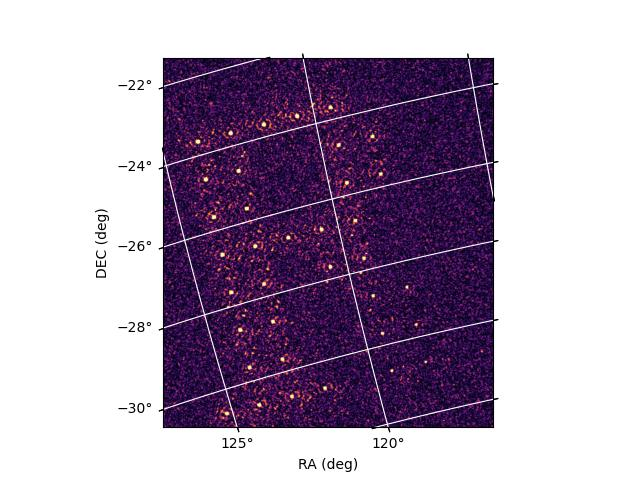
\includegraphics[width=0.9\linewidth]{documentation_figures/cleaned_R.jpg}
    \caption{Plot of WSClean cleaned sky image from simulation output of 1.5\_uvbeam with lines of constant RA and DEC.}
    \label{fig:rclean}
\end{figure}

\begin{figure}[h!]
    \centering
    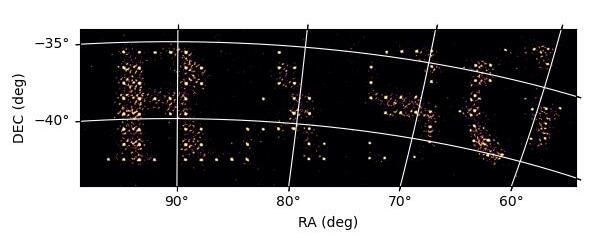
\includegraphics[width=0.9\linewidth]{documentation_figures/cleaned_RASG.jpg}
    \caption{Plot of WSClean cleaned sky image from 1.1\_baseline\_number simulation output with lines of constant RA and DEC.}
    \label{fig:rasgclean}
\end{figure}

\begin{figure}[h!]
    \centering
    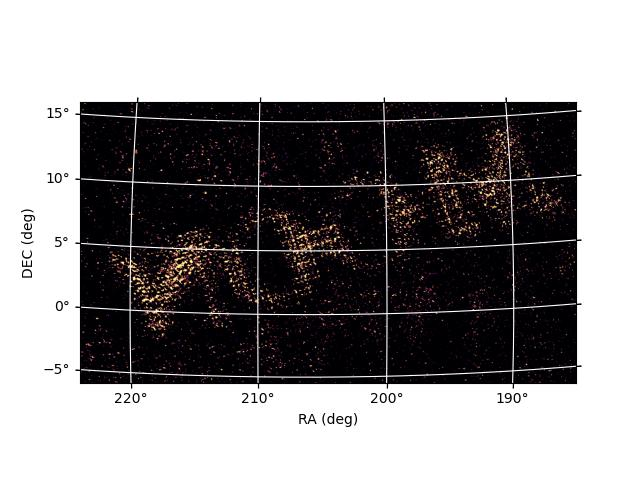
\includegraphics[width=0.9\linewidth]{documentation_figures/cleaned_moon.jpg}
    \caption{A rough WSCleaned image of the sky from simulating 1.8\_lunar. WSClean does not support moon simulations, so the antenna location was set to be on Earth with overlapping RA/DEC sky view, likely causing the lack of source clarity and the reversed and slanted letter orientation.}
    \label{fig:moon}
\end{figure}

\begin{figure}[t!] % "[t!]" placement specifier just for this example
\begin{subfigure}{0.35\textwidth}
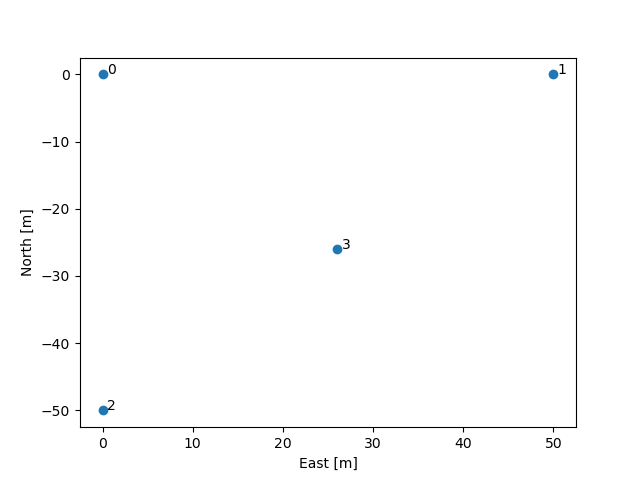
\includegraphics[width=\linewidth]{documentation_figures/bllite_layout.png}
\caption{Plot of bllite layout.} \label{fig:bllite}
\end{subfigure}\hspace*{\fill}
\begin{subfigure}{0.30\textwidth}
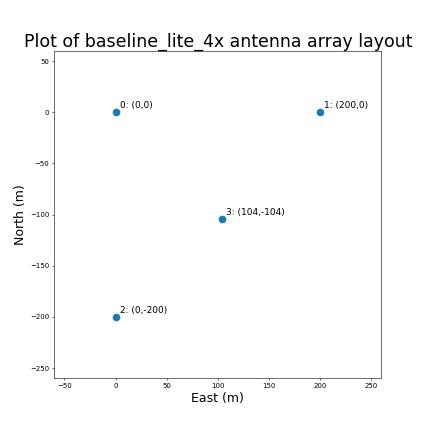
\includegraphics[width=\linewidth]{documentation_figures/rendered_baseline_lite_4x.jpg}
\caption{Plot of bllite 4x layout.}
\label{fig:bllite4x}
\end{subfigure}
\begin{subfigure}{0.30\textwidth}
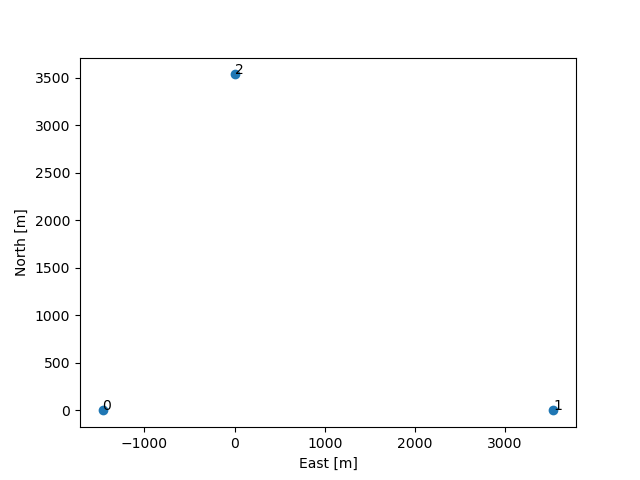
\includegraphics[width=\linewidth]{documentation_figures/5km_triangle_layout.png}
\caption{Plot of 5km triangle layout.}
\label{fig:5kt}
\end{subfigure}

\medskip
\begin{subfigure}{0.40\textwidth}
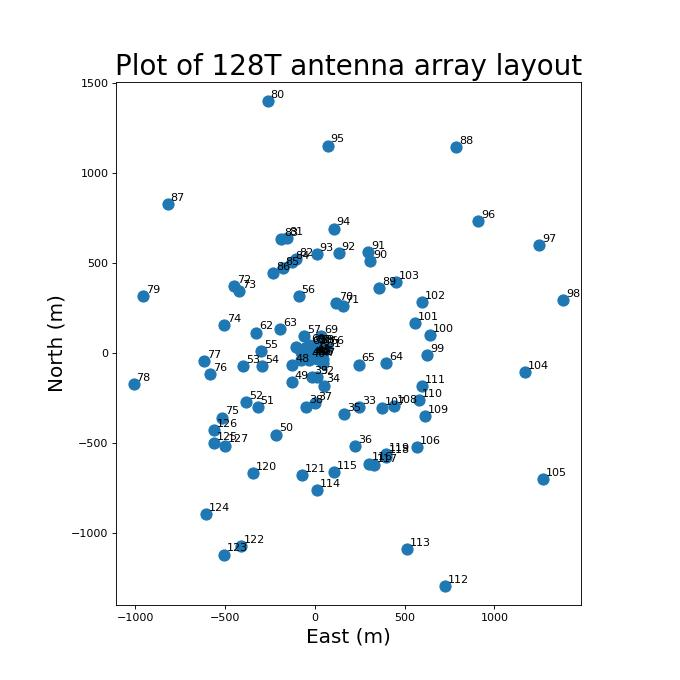
\includegraphics[width=\linewidth]{documentation_figures/rendered_txt_layout_128T.jpg}
\caption{Plot of MWA Phase I (128T) layout (some core sources unlabelled)} \label{fig:mwap1}
\end{subfigure}\hspace*{\fill}
\begin{subfigure}{0.35\textwidth}
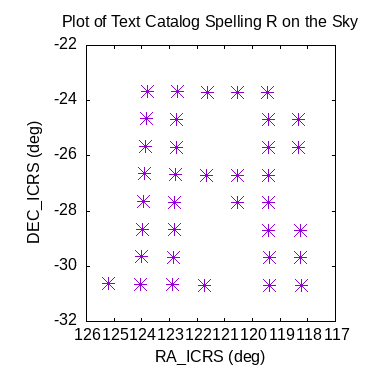
\includegraphics[width=\linewidth]{documentation_figures/R.png}
\caption{Plot of R.txt text catalog created with scripts/im\_to\_catalog.py.} \label{fig:R}
\end{subfigure}

\medskip
\begin{subfigure}{0.40\textwidth}
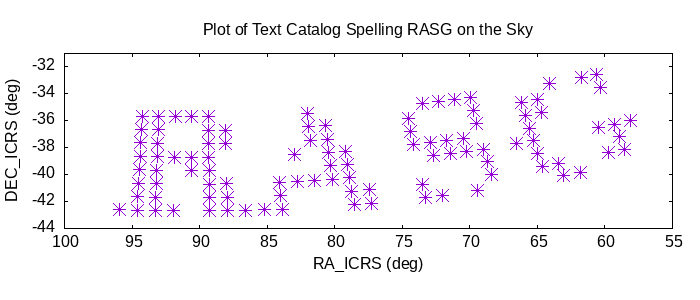
\includegraphics[width=\linewidth]{documentation_figures/RASG.png}
\caption{Plot of RASG.txt text catalog created with scripts/im\_to\_catalog.py.} \label{fig:rasgtxt}
\end{subfigure}\hspace*{\fill}
\begin{subfigure}{0.40\textwidth}
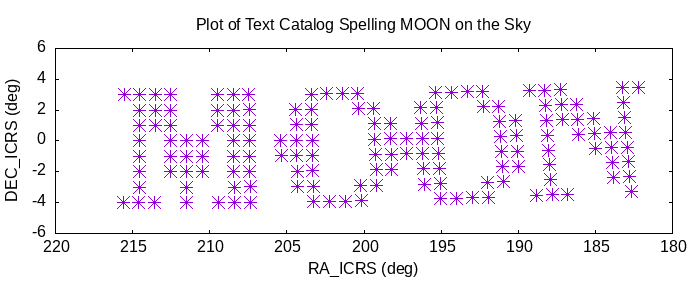
\includegraphics[width=\linewidth]{documentation_figures/MOON.png}
\caption{Plot of MOON.txt text catalog created with scripts/im\_to\_catalog.py.} \label{fig:mooncatalog}
\end{subfigure}

\caption{All array layouts and text catalogs used for reference simulations.} \label{fig:1}
\label{fig:arrays}
\end{figure}

\begin{figure}[htbp]
    \centering
    \begin{subfigure}[b]{1.0\textwidth}
        \centering
        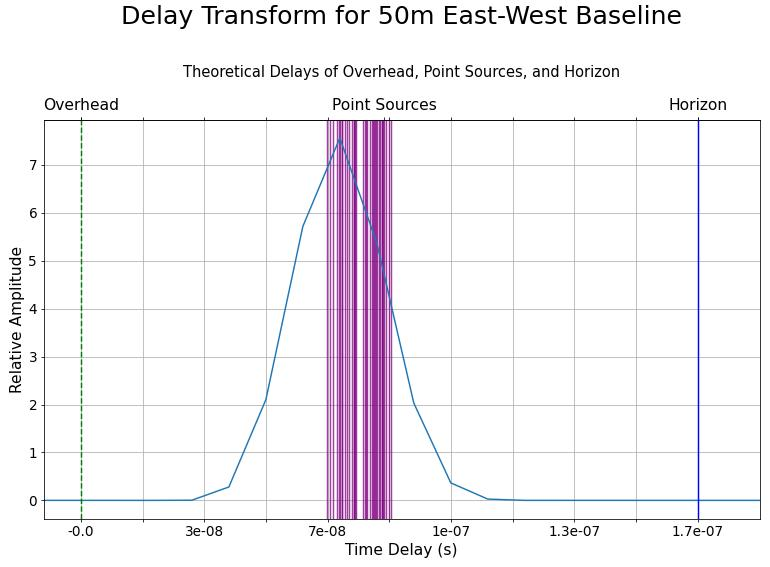
\includegraphics[width=0.62\textwidth]{documentation_figures/delay_transform.jpg}
        \caption{Plot of the delay transform of the 1.3\_frequency\_axis reference simulation output. The sources simulated spelled the letter R on the sky, and were around 30 degrees offset from array zenith in RA. We selected the 'xx' polarization and the (0,1) baseline --- 50 meters East. The theoretical geometric time delays of the sources were calculated and given as the purple lines (labelled Point Sources) in the plot. The other  explicitly labeled delays are the horizon limit -- the maximum possible delay given the baseline configuration -- and overhead, which simply corresponds to no delay. The gaussian beam, and possibly the spectral leakage, causes the peak to be significantly more offset than it would be otherwise. We expect our resolution to be no better than around $\frac{1}{\Delta f} = \frac{1}{10^{8} Hz} = 1*10^{-8} s$, and as such do not resolve individual sources with the current frequency range --- we use a pretty small baseline which additionally reduces sensitivity. We used a Blackman-Harris window function, which also spreads the peak out.}
        \label{fig:delaytransform}
    \end{subfigure}
    \begin{subfigure}[b]{1.0\textwidth}
        \centering
        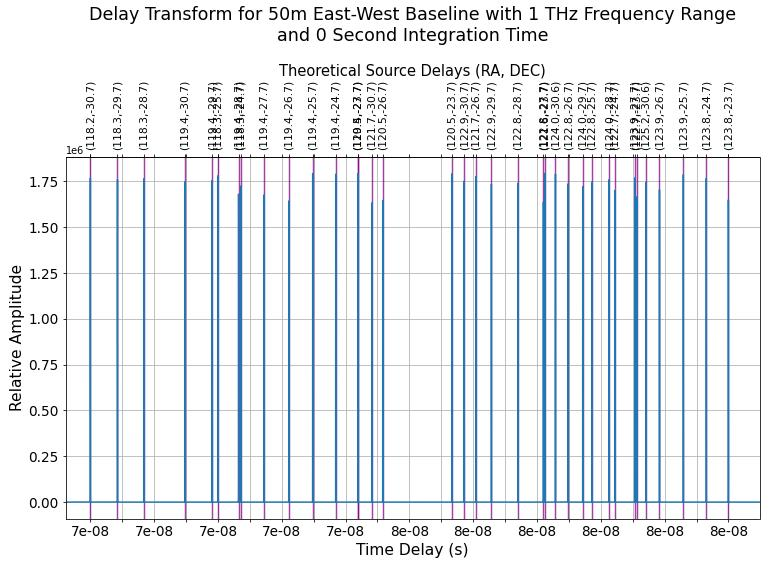
\includegraphics[width=0.62\textwidth]{documentation_figures/theoretical_delay_transform.jpg}
        \caption{Companion plot to Figure \ref{fig:delaytransform} where we simulated the same sources over much wider frequency range -- 1 Terahertz -- and set the integration time to 0 to show an exact match between the theoretical geometric delay for each source and the delay transform peaks. The gaussian beam was also swapped to a uniform beam for better sensitivity. The blue spikes are the delay transform peaks corresponding to each source, and the purple lines are the computed theoretical geometric delays of each source, with the RA and DEC of the source as tick labels. This plot is significantly more zoomed in than Figure \ref{fig:delaytransform} to show the agreement of the computed geometric delays and the delay transform peaks.}
        \label{fig:theorydelay}
    \end{subfigure}
    \caption{Delay transform analysis of 1.3\_frequency\_axis reference simulation with companion plot of same simulation with higher frequency range to show exact match between theoretical and simulated time delays.}
    \label{fig:theorydelays}
\end{figure}

\begin{figure}
    \centering
    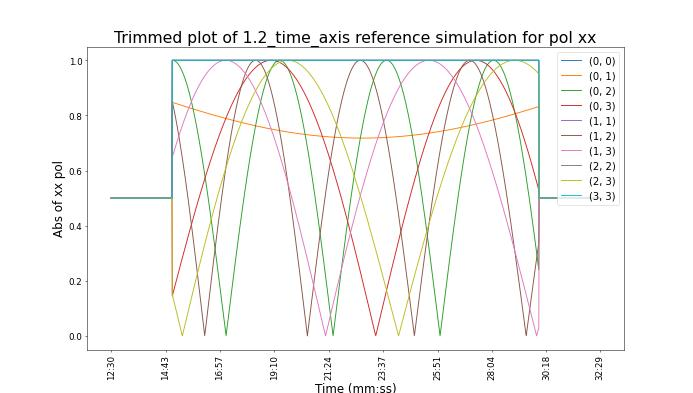
\includegraphics[width=0.85\textwidth]{documentation_figures/new_horizon_baseline_time.jpg}
    \caption{Trimmed plot of the abs of the xx polarization visibilities over time. We drop the first and last 12.5 minutes of the simulation as it is simply a constant line at .5 amplitude as expected. With two sources on the sky, we get the interference pattern discussed where the baselines corresponding to antenna pairs (0,2) and (1,2) oscillate the fastest.}
    \label{fig:4xb}
\end{figure}
\begin{figure}
    \centering
    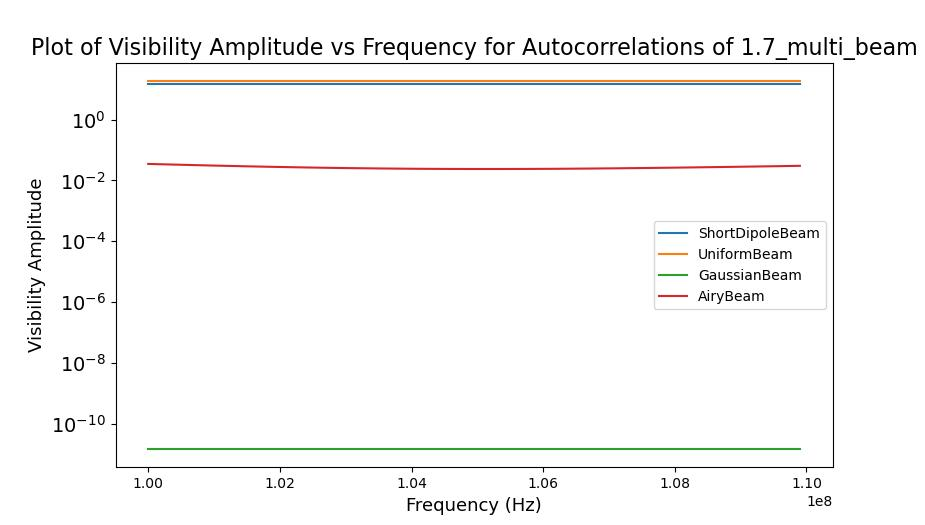
\includegraphics[width=0.85\textwidth]{documentation_figures/autocorrelations.jpg}
    \caption{Plot of visibility amplitude versus time for the autocorrelations of 1.7\_multi\_beam. Note that the y axis has logarithmic scaling. Only the AiryBeam has explicit frequency dependence as expected --- the ShortDipoleBeam and UniformBeam are achromatic while the GaussianBeam is achromatic unless explicitly specified otherwise. The uniform beam has the largest visibility as it has full and identical response in all directions, with the ShortDipoleBeam below it. The AiryBeam and GaussianBeam have much lower amplitude as expected as they both fall off exponentially with the GaussianBeam having the lowest amplitude. The sources on the sky for this simulation were those of Figure \ref{fig:R}: spelling the letter R shifted 30 degrees from overhead.}
    \label{fig:autocorr}
\end{figure}

\end{document}


% NOTES:

% \Delta f = 100 MHz
% \delta f = 10 KHz
% \Delta \tau = \frac{1}{\delta f}
% \delta \tau = \frac{1}{\Delta f}
%
% TO TRY: bigger beam, longer bandwidth, freq resolution the same, maybe a line of sources E-W every 5 degrees horizon to horizon

% can use blown up array also for better resolution

% sensible fringes: nicely oscillatory given we have enough frequency bandwidth / longer baselines, and time delays are nicely constrained to be in the horizon delay
